\documentclass[tikz, border=10pt]{standalone}
\usepackage{tikz}
\usetikzlibrary{shapes.geometric, arrows.meta, positioning, fit, backgrounds, calc}

\begin{document}

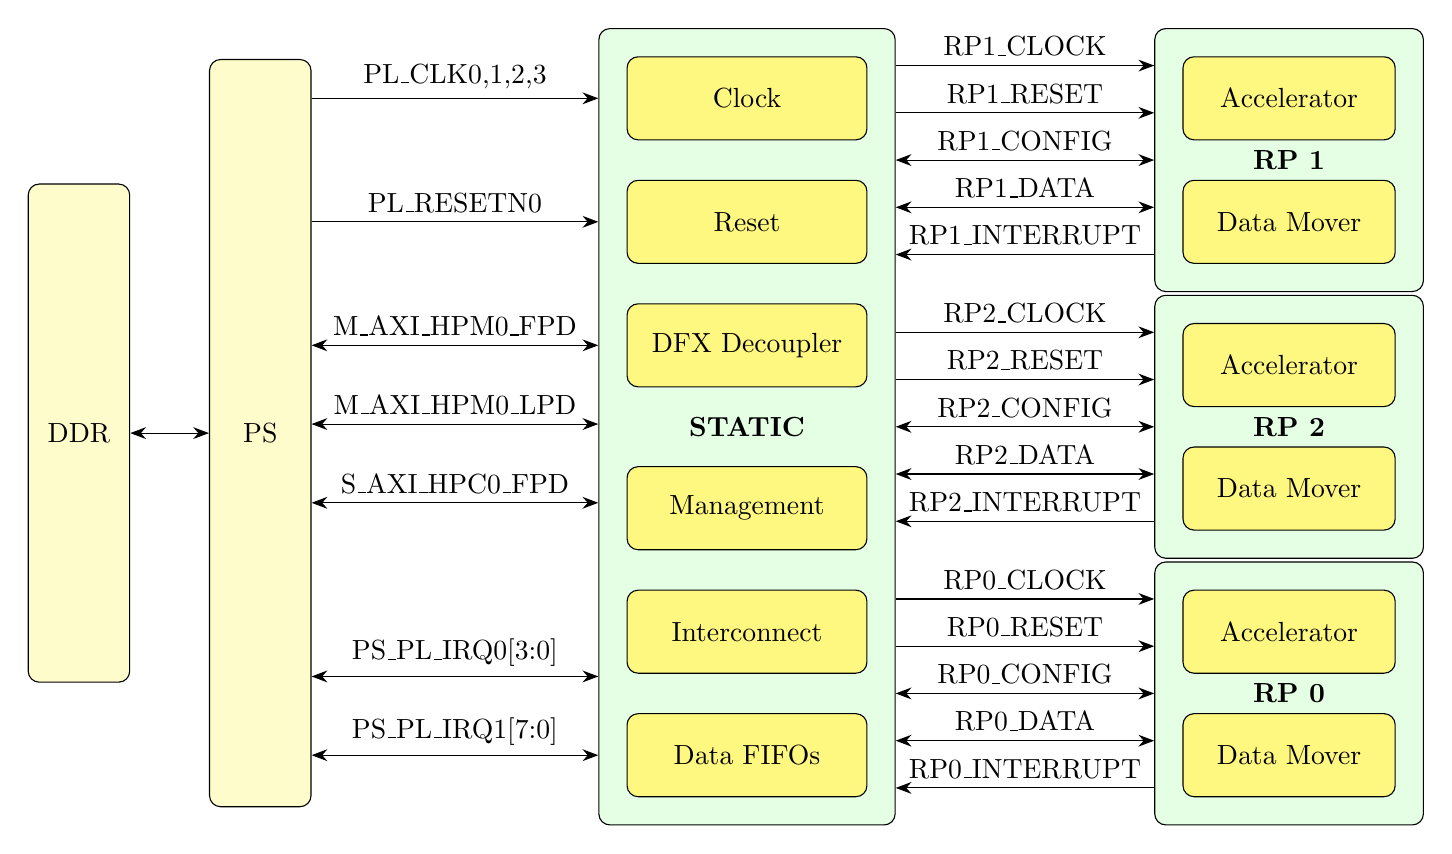
\begin{tikzpicture}[
    auto,
    block/.style={rectangle, draw, fill=yellow!20,
        text width=10em, text centered, rounded corners, minimum height=4em},
    line/.style={draw, -{Stealth[length=2mm, width=1.5mm]}},
    double_line/.style={draw, {Stealth[length=2mm, width=1.5mm]}-{Stealth[length=2mm, width=1.5mm]}},
    small_block/.style={rectangle, draw, fill=yellow!50,
        text width=8em, text centered, rounded corners, minimum height=3em},
    group_block/.style={rectangle, draw, fill=green!10, rounded corners, inner sep=10pt},
    rp_internal_block/.style={rectangle, draw, fill=yellow!50, rounded corners, minimum height=3em, text width=7em, text centered}
]

% Nodes on the left
\node[block, minimum height=18em, text width=3em] (ddr) {DDR};
\node[block, minimum height=27em, right=1cm of ddr, text width=3em] (ps) {PS};

% Central static block components
\node[small_block, right=4cm of ps.north east, yshift=-0.5cm] (clock) {Clock};
\node[small_block, below=0.5cm of clock] (reset) {Reset};
\node[small_block, below=0.5cm of reset] (dfx_decoupler) {DFX Decoupler};
\node[small_block, below=1cm of dfx_decoupler] (static_management) {Management};
\node[small_block, below=0.5cm of static_management] (interconnect) {Interconnect};
\node[small_block, below=0.5cm of interconnect] (ir_buffers) {Data FIFOs};

% Fit a block around the central static components
\begin{scope}[on background layer]
    \node[group_block, fit=(clock) (reset) (dfx_decoupler) (static_management) (interconnect) (ir_buffers), label={center:\textbf{STATIC}}] (static_group) {};
\end{scope}

% RP1 components
\node[rp_internal_block, right=4cm of clock, anchor=west] (rp1_accel) {Accelerator};
\node[rp_internal_block, below=0.5cm of rp1_accel] (rp1_dm) {Data Mover};

% Fit a block around RP1 components
\begin{scope}[on background layer]
    \node[group_block, fit=(rp1_accel) (rp1_dm), label={center:\textbf{RP 1}}] (rp1_group) {};
\end{scope}

% RP0 components
\node[rp_internal_block, right=4cm of dfx_decoupler, anchor=west, yshift=-1cm-2.33em] (rp2_dm) {Data Mover};
\node[rp_internal_block, above=0.5cm of rp2_dm] (rp2_accel) {Accelerator};

% Fit a block around RP0 components
\begin{scope}[on background layer]
    \node[group_block, fit=(rp2_accel) (rp2_dm), label={center:\textbf{RP 2}}] (rp2_group) {};
\end{scope}


% RP0 components
\node[rp_internal_block, right=4cm of ir_buffers, anchor=west] (rp0_dm) {Data Mover};
\node[rp_internal_block, above=0.5cm of rp0_dm] (rp0_accel) {Accelerator};

% Fit a block around RP0 components
\begin{scope}[on background layer]
    \node[group_block, fit=(rp0_accel) (rp0_dm), label={center:\textbf{RP 0}}] (rp0_group) {};
\end{scope}


% Connections from PS to Static Group
\path [line] (ps.east |- clock.west) -- (static_group.west |- clock.west) node[midway, above] {PL\_CLK0,1,2,3};
\path [line] (ps.east |- reset.west) -- (static_group.west |- reset.west) node[midway, above] {PL\_RESETN0};
\path [double_line] (ps.east |- dfx_decoupler.west) -- (static_group.west |- dfx_decoupler.west) node[midway, above] {M\_AXI\_HPM0\_FPD};
\path [double_line] ($(ps.east |- dfx_decoupler.west) + (0,-1cm)$) -- ($(static_group.west |- dfx_decoupler.west) + (0,-1cm)$) node[midway, above] {M\_AXI\_HPM0\_LPD};
\path [double_line] ($(ps.east |- dfx_decoupler.west) + (0,-2cm)$) -- ($(static_group.west |- dfx_decoupler.west) + (0,-2cm)$) node[midway, above] {S\_AXI\_HPC0\_FPD};
\path [double_line] ($(ps.east |- ir_buffers.west) + (0,1cm)$) -- ($(static_group.west |- ir_buffers.west) + (0,1cm)$) node[midway, above] {PS\_PL\_IRQ0[3:0]};
\path [double_line] (ps.east |- ir_buffers.west) -- (static_group.west |- ir_buffers.west) node[midway, above] {PS\_PL\_IRQ1[7:0]};


% Connections from Static Group to RP1
\path [line] ($(static_group.east |- rp1_group) + (0,1.2cm)$) -- ($(rp1_group.west |- rp1_group) + (0,1.2cm)$) node[midway, above] {RP1\_CLOCK};
\path [line] ($(static_group.east |- rp1_group) + (0,0.6cm)$) -- ($(rp1_group.west |- rp1_group) + (0,0.6cm)$) node[midway, above] {RP1\_RESET};
\path [double_line] (static_group.east |- rp1_group) -- (rp1_group.west |- rp1_group) node[midway, above] {RP1\_CONFIG};
\path [double_line] ($(static_group.east |- rp1_group) + (0,-0.6cm)$) -- ($(rp1_group.west |- rp1_group) + (0,-0.6cm)$) node[midway, above] {RP1\_DATA};
\path [line] ($(rp1_group.west |- rp1_group) + (0,-1.2cm)$) -- ($(static_group.east |- rp1_group) + (0,-1.2cm)$) node[midway, above] {RP1\_INTERRUPT};


% Connections from Static Group to RP2
\path [line] ($(static_group.east |- rp2_group) + (0,1.2cm)$) -- ($(rp2_group.west |- rp2_group) + (0,1.2cm)$) node[midway, above] {RP2\_CLOCK};
\path [line] ($(static_group.east |- rp2_group) + (0,0.6cm)$) -- ($(rp2_group.west |- rp2_group) + (0,0.6cm)$) node[midway, above] {RP2\_RESET};
\path [double_line] (static_group.east |- rp2_group) -- (rp2_group.west |- rp2_group) node[midway, above] {RP2\_CONFIG};
\path [double_line] ($(static_group.east |- rp2_group) + (0,-0.6cm)$) -- ($(rp2_group.west |- rp2_group) + (0,-0.6cm)$) node[midway, above] {RP2\_DATA};
\path [line] ($(rp2_group.west |- rp2_group) + (0,-1.2cm)$) -- ($(static_group.east |- rp2_group) + (0,-1.2cm)$) node[midway, above] {RP2\_INTERRUPT};


% Connections from Static Group to RP0
\path [line] ($(static_group.east |- rp0_group) + (0,1.2cm)$) -- ($(rp0_group.west |- rp0_group) + (0,1.2cm)$) node[midway, above] {RP0\_CLOCK};
\path [line] ($(static_group.east |- rp0_group) + (0,0.6cm)$) -- ($(rp0_group.west |- rp0_group) + (0,0.6cm)$) node[midway, above] {RP0\_RESET};
\path [double_line] (static_group.east |- rp0_group) -- (rp0_group.west |- rp0_group) node[midway, above] {RP0\_CONFIG};
\path [double_line] ($(static_group.east |- rp0_group) + (0,-0.6cm)$) -- ($(rp0_group.west |- rp0_group) + (0,-0.6cm)$) node[midway, above] {RP0\_DATA};
\path [line] ($(rp0_group.west |- rp0_group) + (0,-1.2cm)$) -- ($(static_group.east |- rp0_group) + (0,-1.2cm)$) node[midway, above] {RP0\_INTERRUPT};


% Connection DDR to PS
\path [double_line] (ddr.east) -- (ps.west);

\end{tikzpicture}

\end{document}
